%%%% CAPÍTULO — RESULTADOS
%%
\chapter{Resultados}\label{cap:resultados}

Este capítulo consolida o que foi alcançado após as etapas de desenvolvimento descritas no Capítulo~\ref{cap:desenvolvimento}. O foco não é repetir o cronograma de implementação, mas apresentar a síntese frente aos objetivos, a evolução do modelo de dados e do produto em relação à versão legada, capturas da interface entregue, indicadores verificáveis do repositório (incluindo a atividade no \textit{GitHub} institucional) e a situação da entrega operacional.


\section{Síntese em relação aos objetivos}\label{sec:resultados-objetivos}

Ao término do ciclo documentado nesta monografia, consolidaram-se os principais resultados do trabalho em relação ao objetivo geral (Seção~\ref{subsec:objetivoGeral}) e aos objetivos específicos (Seção~\ref{subsec:objetivoEspecificos}). A Tabela~\ref{tab:objetivos-resultados} resume, de forma sintética, o atendimento a cada meta e indica onde a evidência correspondente é detalhada no texto. Evoluções que extrapolam o escopo deste ciclo são discutidas nas limitações e nos trabalhos futuros (Seções~\ref{sec:conclusao-limitacoes} e~\ref{sec:conclusao-trabalhos-futuros}).

\begin{table}[H]
    \centering
    \caption{Síntese dos objetivos específicos e dos resultados alcançados.}
    \label{tab:objetivos-resultados}
    \begin{tabularx}{\textwidth}{@{}p{0.36\textwidth}Xp{0.14\textwidth}@{}}
        \toprule
        \textbf{Objetivo específico} & \textbf{Principal evidência no trabalho} & \textbf{Situação} \\
        \midrule
        Versionamento e padrões no GitHub &
        Seções~\ref{sec:dev-gitflow} e~\ref{sec:dev-requisitos} &
        Atendido \\
        Ambientes de desenvolvimento, teste e produção &
        Seções~\ref{sec:dev-infra},~\ref{sec:dev-deploy} e~\ref{sec:resultados-operacional} &
        Atendido \\
        Refatoração do código existente &
        Seções~\ref{sec:dev-refatoracao} e~\ref{sec:resultados-modelo-dados} &
        Atendido \\
        Testes automatizados &
        Seção~\ref{sec:dev-testes}; Seção~\ref{sec:resultados-indicadores} &
        Atendido \\
        Novas funcionalidades do E-Museu &
        Seção~\ref{sec:dev-funcionalidades} &
        Atendido \\
        Padrões de projeto e boas práticas &
        Seções~\ref{sec:dev-refatoracao} e~\ref{sec:dev-funcionalidades}; Capítulo~\ref{cap-referencial-teorico} &
        Atendido \\
        \bottomrule
    \end{tabularx}
    \caption*{\textbf{Fonte:} Autoria própria.}
\end{table}


\section{Evolução do modelo de dados}\label{sec:resultados-modelo-dados}

A Figura~\ref{fig:emuseu-bd-evolucao} resume o esquema relacional da versão entregue, com destaque para alterações em relação ao legado descrito por \citeonline{gonzaga2024} e às migrações documentadas no Capítulo~\ref{cap:desenvolvimento}. Entidades e colunas removidas aparecem riscadas; criações ou renomeações recentes, em verde; campos ou tabelas previstos para internacionalização ou localização, em laranja; estruturas ligadas a traduções assistidas no painel, em roxo.

\begin{figure}[htb]
    \centering
    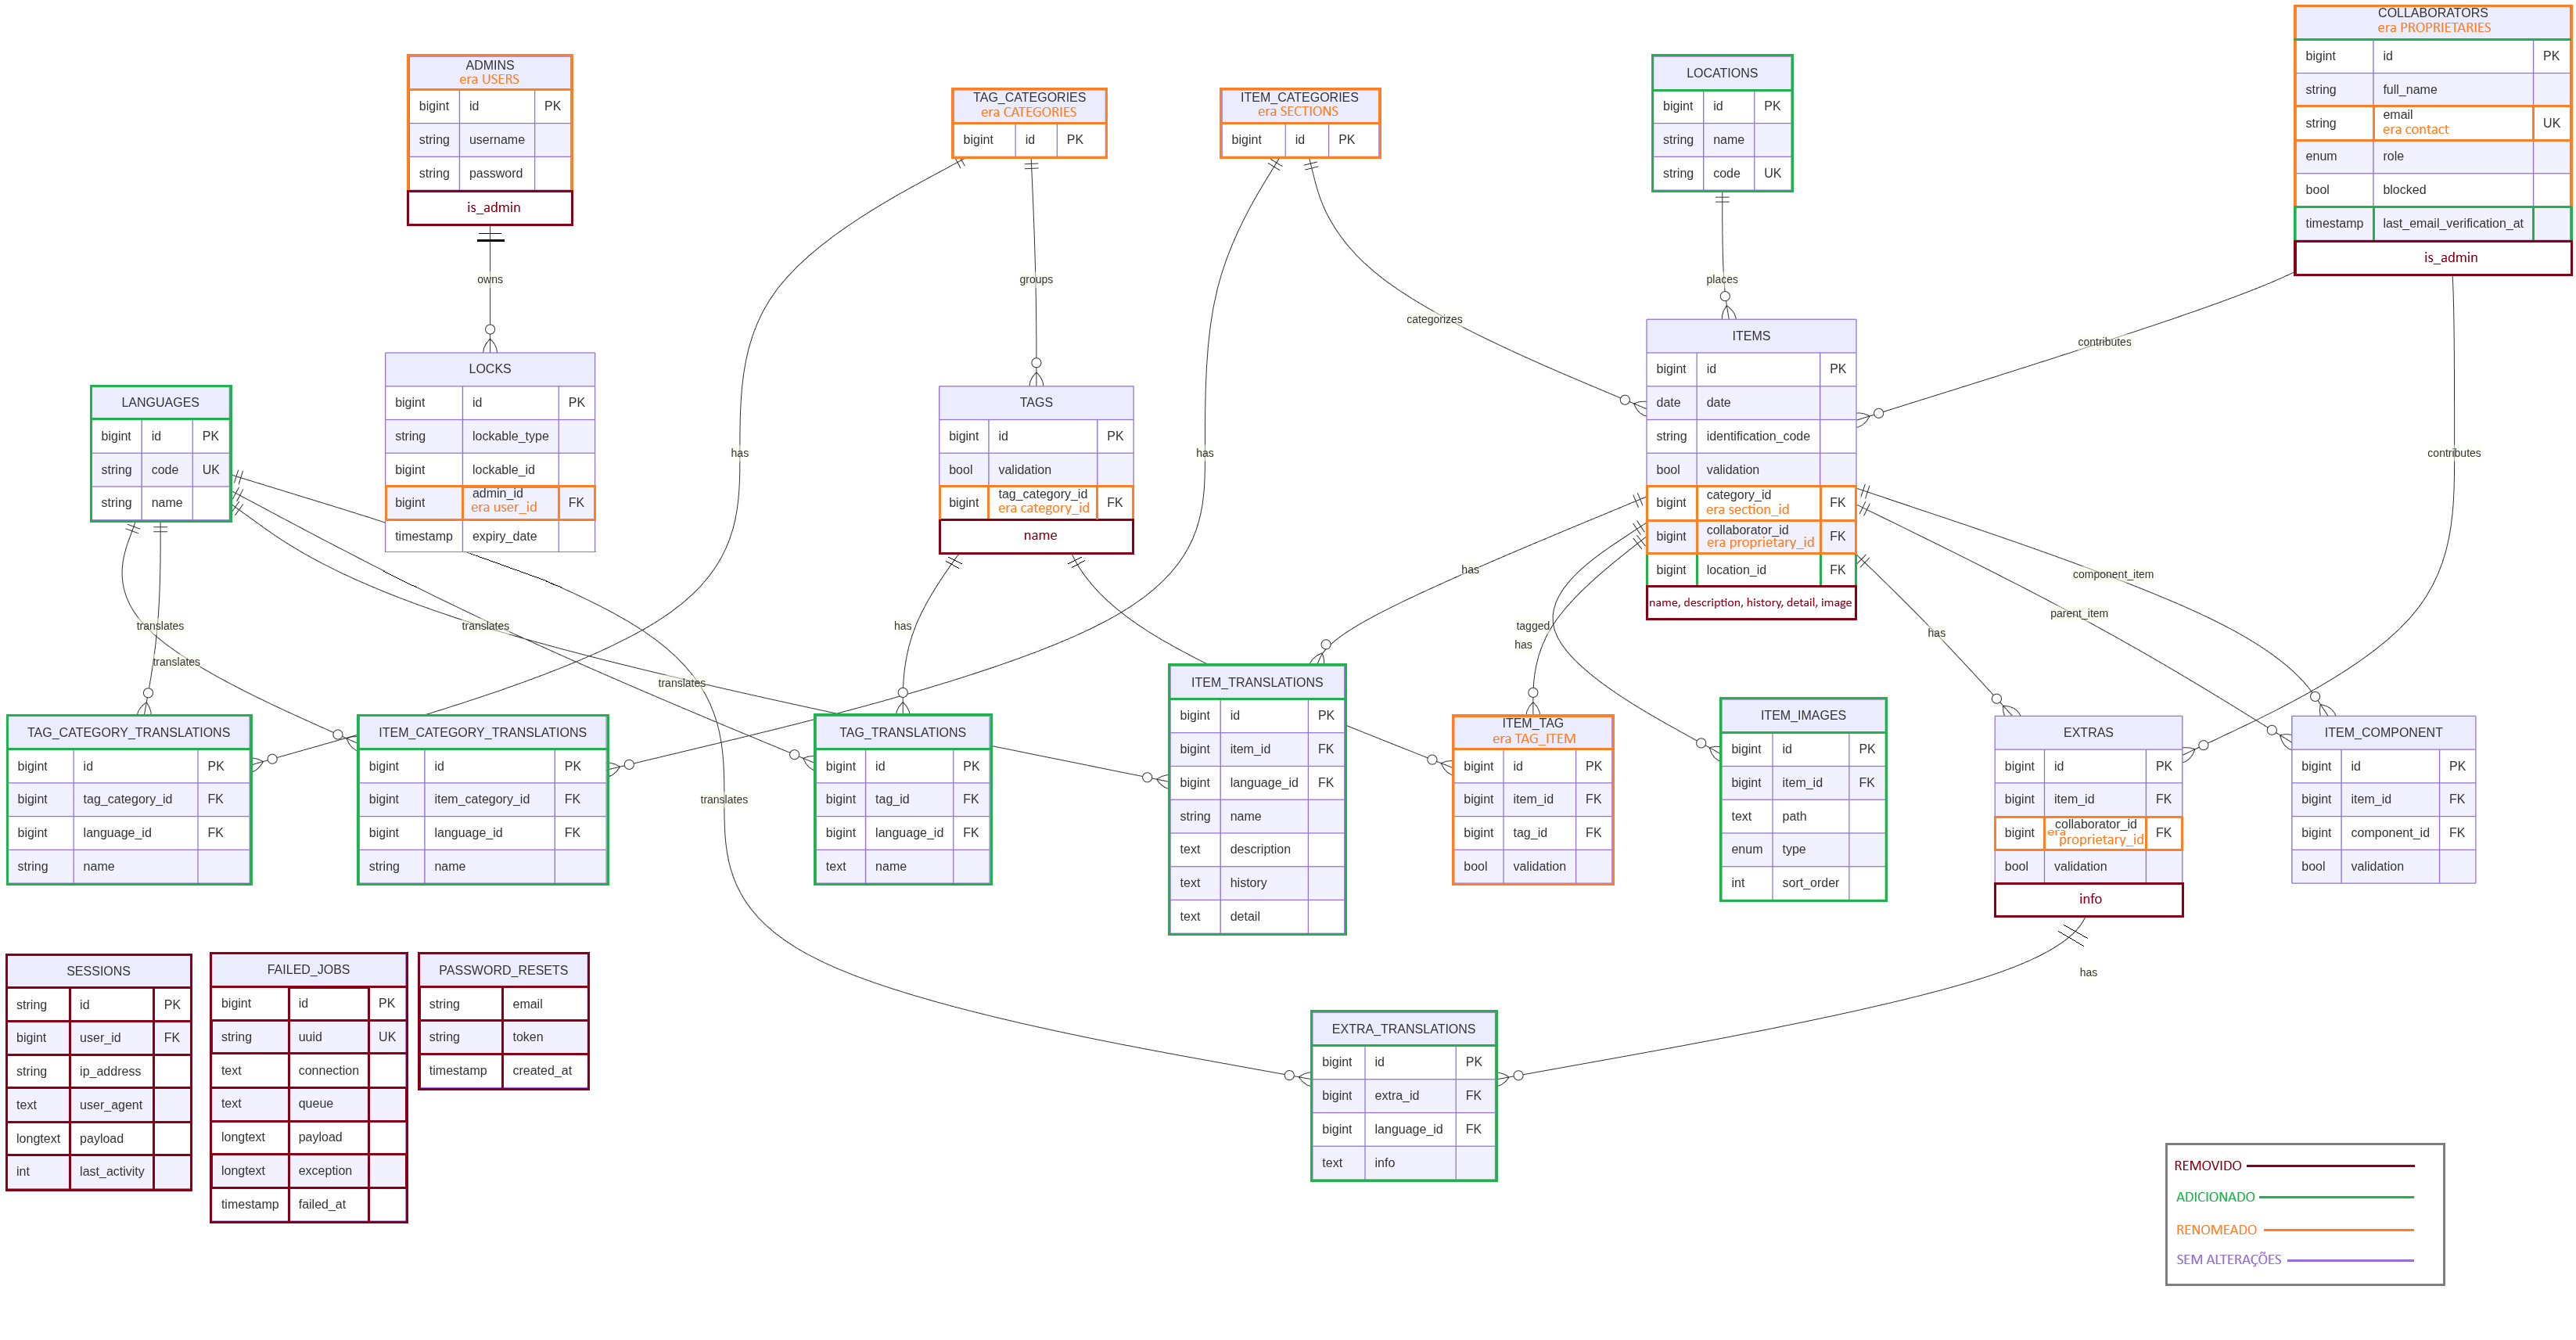
\includegraphics[width=\textwidth]{figuras/emuseu-banco-de-dados.png}
    \caption{Modelo relacional do E-Museu refatorado (visão consolidada).}
    \label{fig:emuseu-bd-evolucao}
    \caption*{\textbf{Fonte:} Autoria própria. \textbf{Legenda:} removido (riscado); novo ou renomeado (verde); previsto para i18n ou \texttt{locations} (laranja); suporte a traduções no painel (roxo).}
\end{figure}

Em fevereiro de 2026, a reorganização por domínios e a adoção de armazenamento por proxy (Subseção~\ref{sec:dev-storage-minio}) antecederam a \textit{release} \texttt{3.0.0-beta}. Em março, o pacote de renomeações (Subseção~\ref{sec:dev-refatoracao-vocabulario}) alinhou o vocabulário físico do banco ao das pastas de aplicação: \texttt{users} para \texttt{admins}, \texttt{sections} para \texttt{item\_categories}, \texttt{proprietaries} para \texttt{collaborators}, \texttt{categories} para \texttt{tag\_categories}, além da tabela \texttt{item\_images} e da associação \texttt{item\_tag}. A \textit{release} \texttt{4.0.0-beta} promoveu esse conjunto a \texttt{main}.

Entregas de abril de 2026 (internacionalização completa do acervo, domínio \texttt{Location} e atualização para Laravel~13, Seção~\ref{sec:dev-stack-upgrade}) acrescentaram ou consolidaram tabelas e colunas indicadas em laranja e roxo na figura; o detalhamento cronológico permanece no Capítulo~\ref{cap:desenvolvimento}, enquanto esta seção fixa o estado final do modelo para leitura comparativa.


\section{Evolução do software em relação ao legado}\label{sec:resultados-evolucao-software}

Em relação à versão descrita por \citeonline{gonzaga2024}, o E-Museu refatorado passou a operar com ambientes distintos de desenvolvimento local, \textit{staging} e produção; pilha atualizada (\acrshort{php}~8.5, Laravel~13); organização por domínios sob \texttt{app/Domain/}; armazenamento de mídia em objeto (MinIO) com URLs servidas por proxy; dezenas de testes automatizados de fluxo e integração; \textit{pipeline} de qualidade com Pint, PHPStan e testes no \textit{GitHub Actions}; e documentação de fluxo de desenvolvimento no perfil \textit{full} do Gitflow \cite{gitflowdoc}.

A base legada concentrava regras em controladores extensos, vocabulário misto (\texttt{users}, \texttt{proprietaries}, \texttt{sections}) e pouca cobertura de testes. A versão atual distribui regras em serviços, \textit{Actions} e \textit{Form Requests}, expõe \textit{endpoints} JSON por domínio e removeu fluxos não utilizados (registro público genérico, assistente ``Ada''). Funcionalidades priorizadas no MoSCoW (internacionalização, múltiplas imagens, QR Code, Turnstile, tradução assistida no painel) integram-se a esse núcleo; requisitos de menor prioridade permanecem fora deste ciclo (Seção~\ref{sec:dev-func-escopo-nao}).


\subsection{Interface pública e painel administrativo}\label{sec:resultados-interface}

A identidade visual e o \textit{layout} geral da página inicial e do painel administrativo permanecem próximos aos da versão de \citeonline{gonzaga2024}: a restilização ampla da interface não entrou no escopo deste TCC, cujo foco foi refatoração, infraestrutura, testes e funcionalidades de acervo descritas no Capítulo~\ref{cap:desenvolvimento}. Ainda assim, as Figuras~\ref{fig:emuseu-home} e~\ref{fig:emuseu-admin} registram como o sistema se apresenta em produção após as entregas, para o leitor visualizar o produto final sem depender do site.

A Figura~\ref{fig:emuseu-home} mostra a página inicial pública em \url{https://e-museu.gp.utfpr.edu.br/home}: cabeçalho com navegação (\textit{Explorar}, contribuição, sobre), seletor de idioma e bloco institucional sobre o museu virtual de informática da parceria \acrshort{utfpr}/\acrshort{unicentro}. As mudanças mais visíveis ao visitante concentram-se no catálogo e nos fluxos novos (internacionalização do acervo, contribuição com verificação por e-mail, Turnstile), ilustrados nas Seções~\ref{sec:dev-funcionalidades} e~\ref{sec:dev-funcionalidades-i18n}, e não na \textit{landing page}.

\begin{figure}[H]
    \centering
    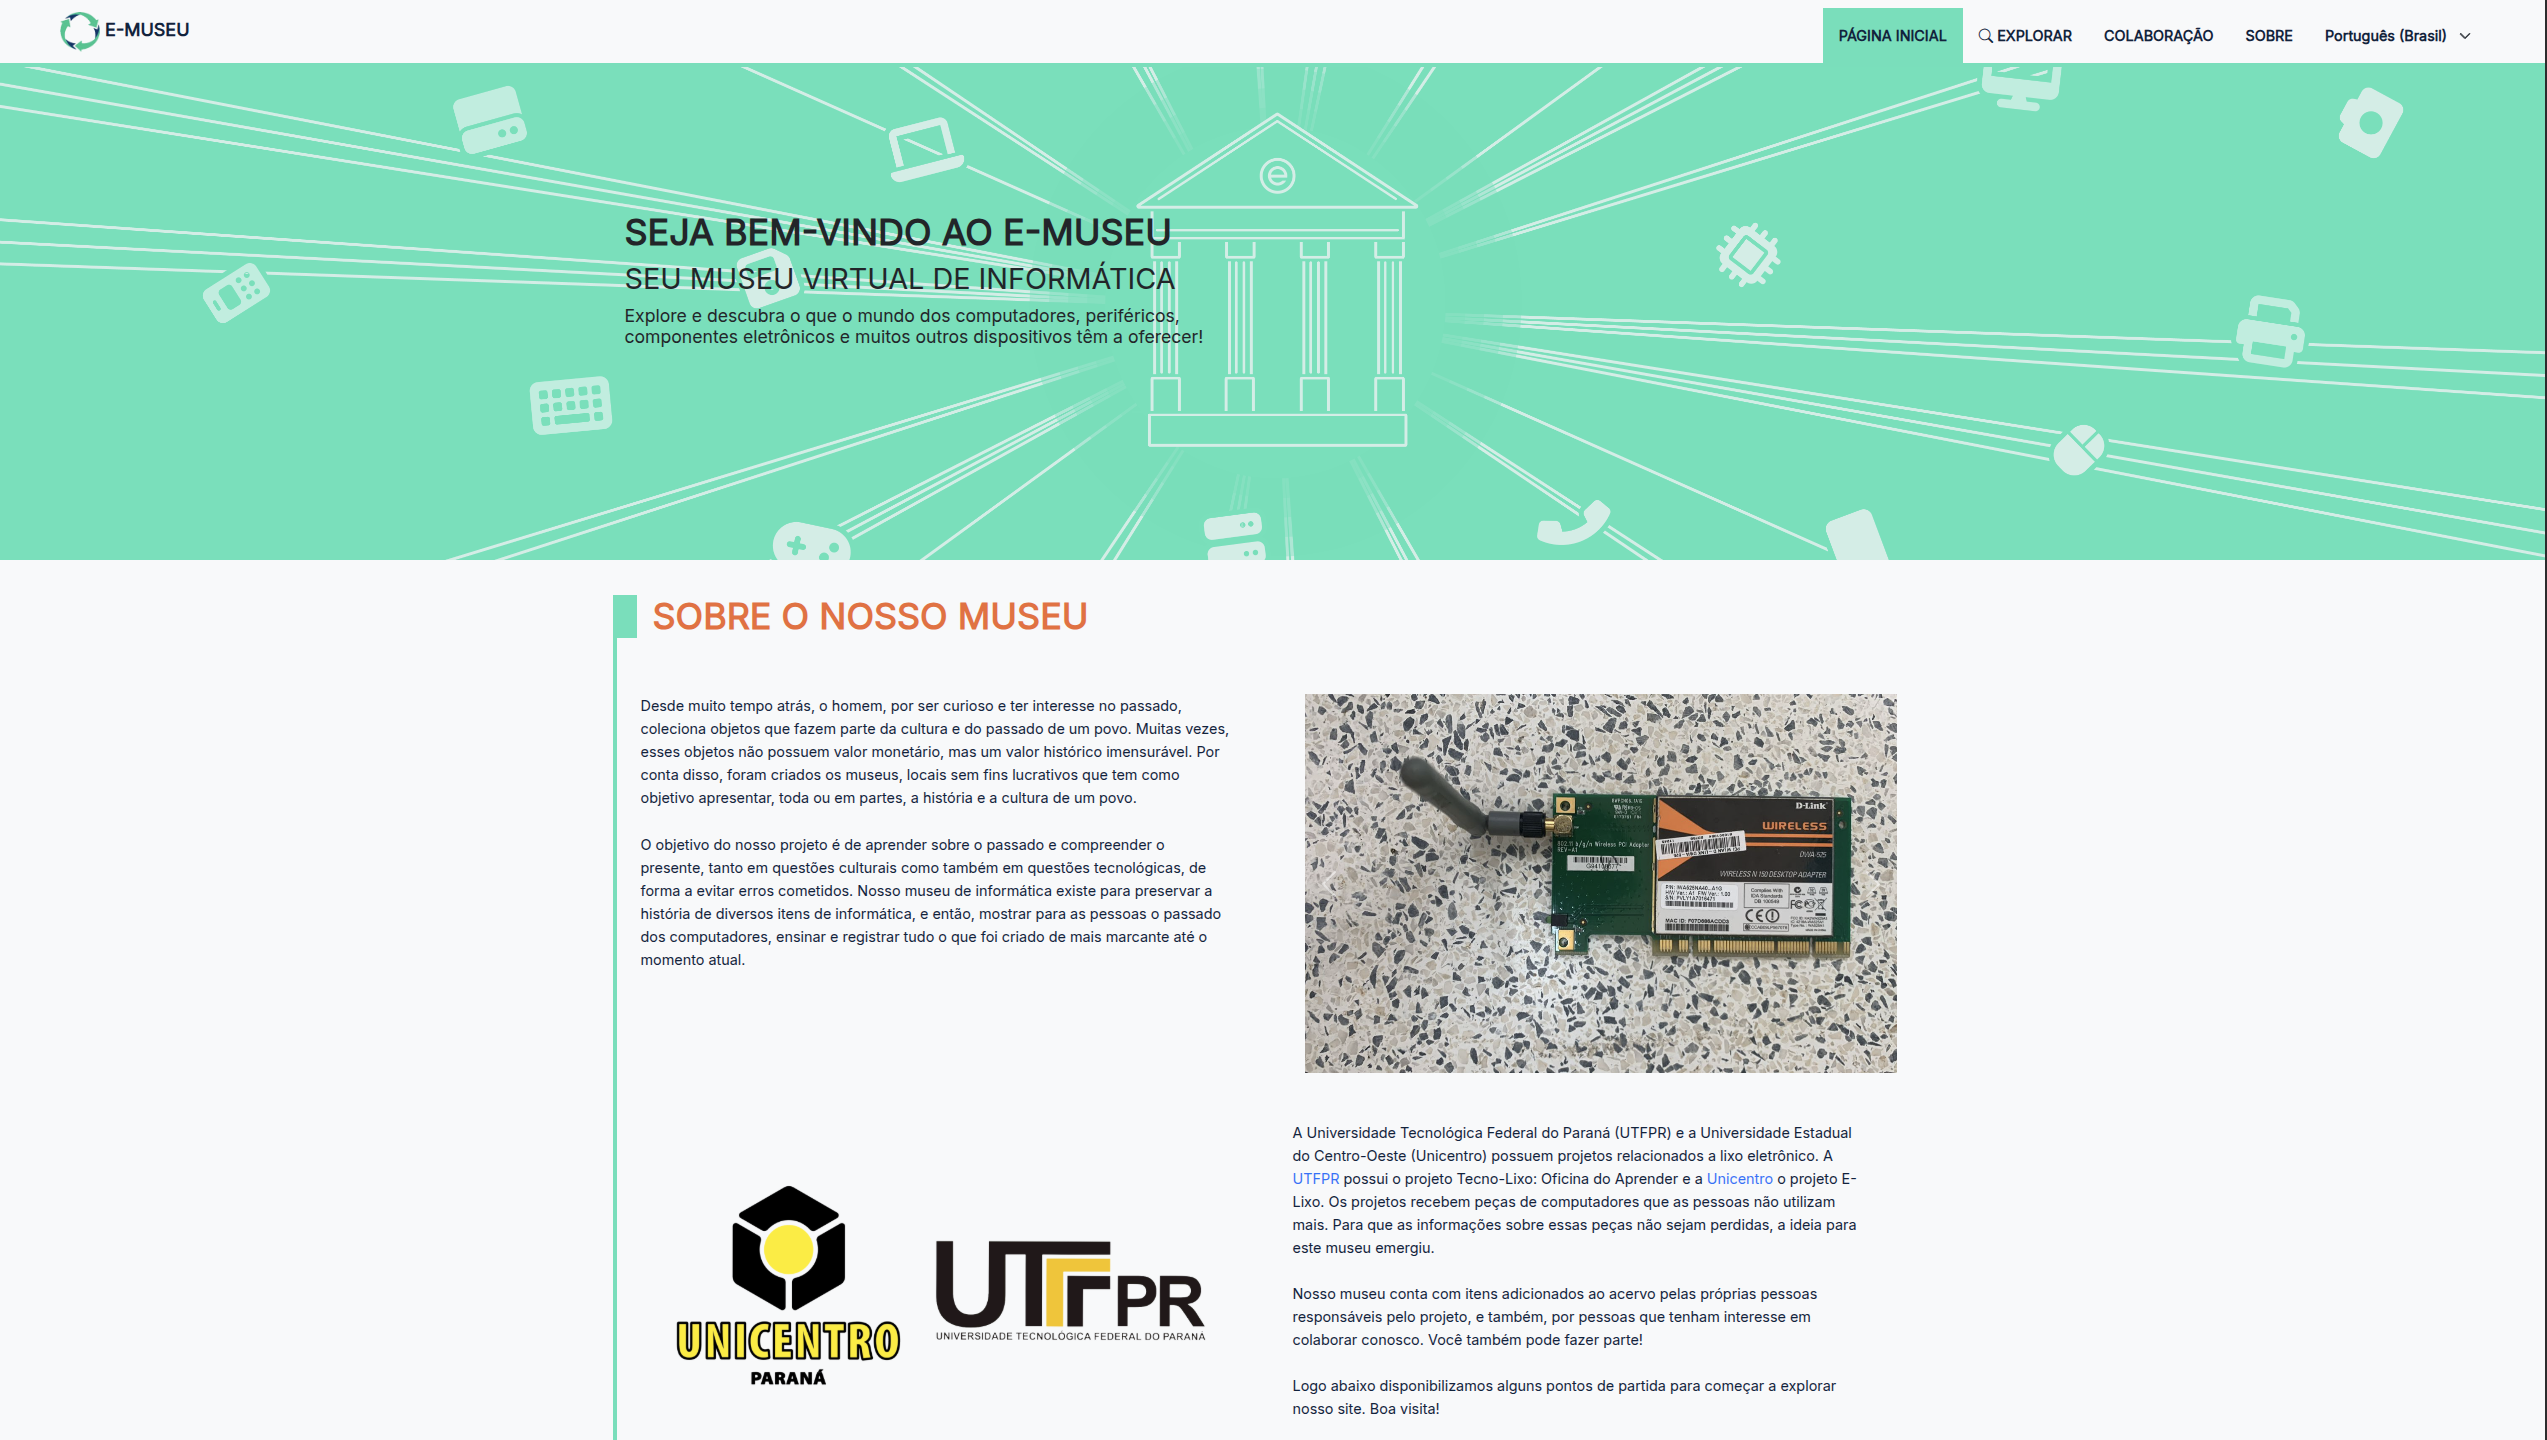
\includegraphics[width=\textwidth]{figuras/emuseu-home.png}
    \caption{Página inicial do E-Museu em produção (\url{https://e-museu.gp.utfpr.edu.br/home}).}
    \label{fig:emuseu-home}
    \caption*{\textbf{Fonte:} Autoria própria (produção, maio/2026).}
\end{figure}

A Figura~\ref{fig:emuseu-admin} apresenta o painel administrativo na listagem de itens do acervo (\url{https://e-museu.gp.utfpr.edu.br/admin/catalog/items}): menu lateral com entidades alinhadas ao modelo refatorado (categorias de item, colaboradores, administradores, entre outras), busca por campo, tabela com código de identificação, localização, validação e ações de visualização, edição e exclusão. O vocabulário do menu reflete renomeações do banco (Seção~\ref{sec:resultados-modelo-dados}); telas específicas de tradução assistida, múltiplas imagens e QR Code aparecem no Capítulo~\ref{cap:desenvolvimento}.

\begin{figure}[H]
    \centering
    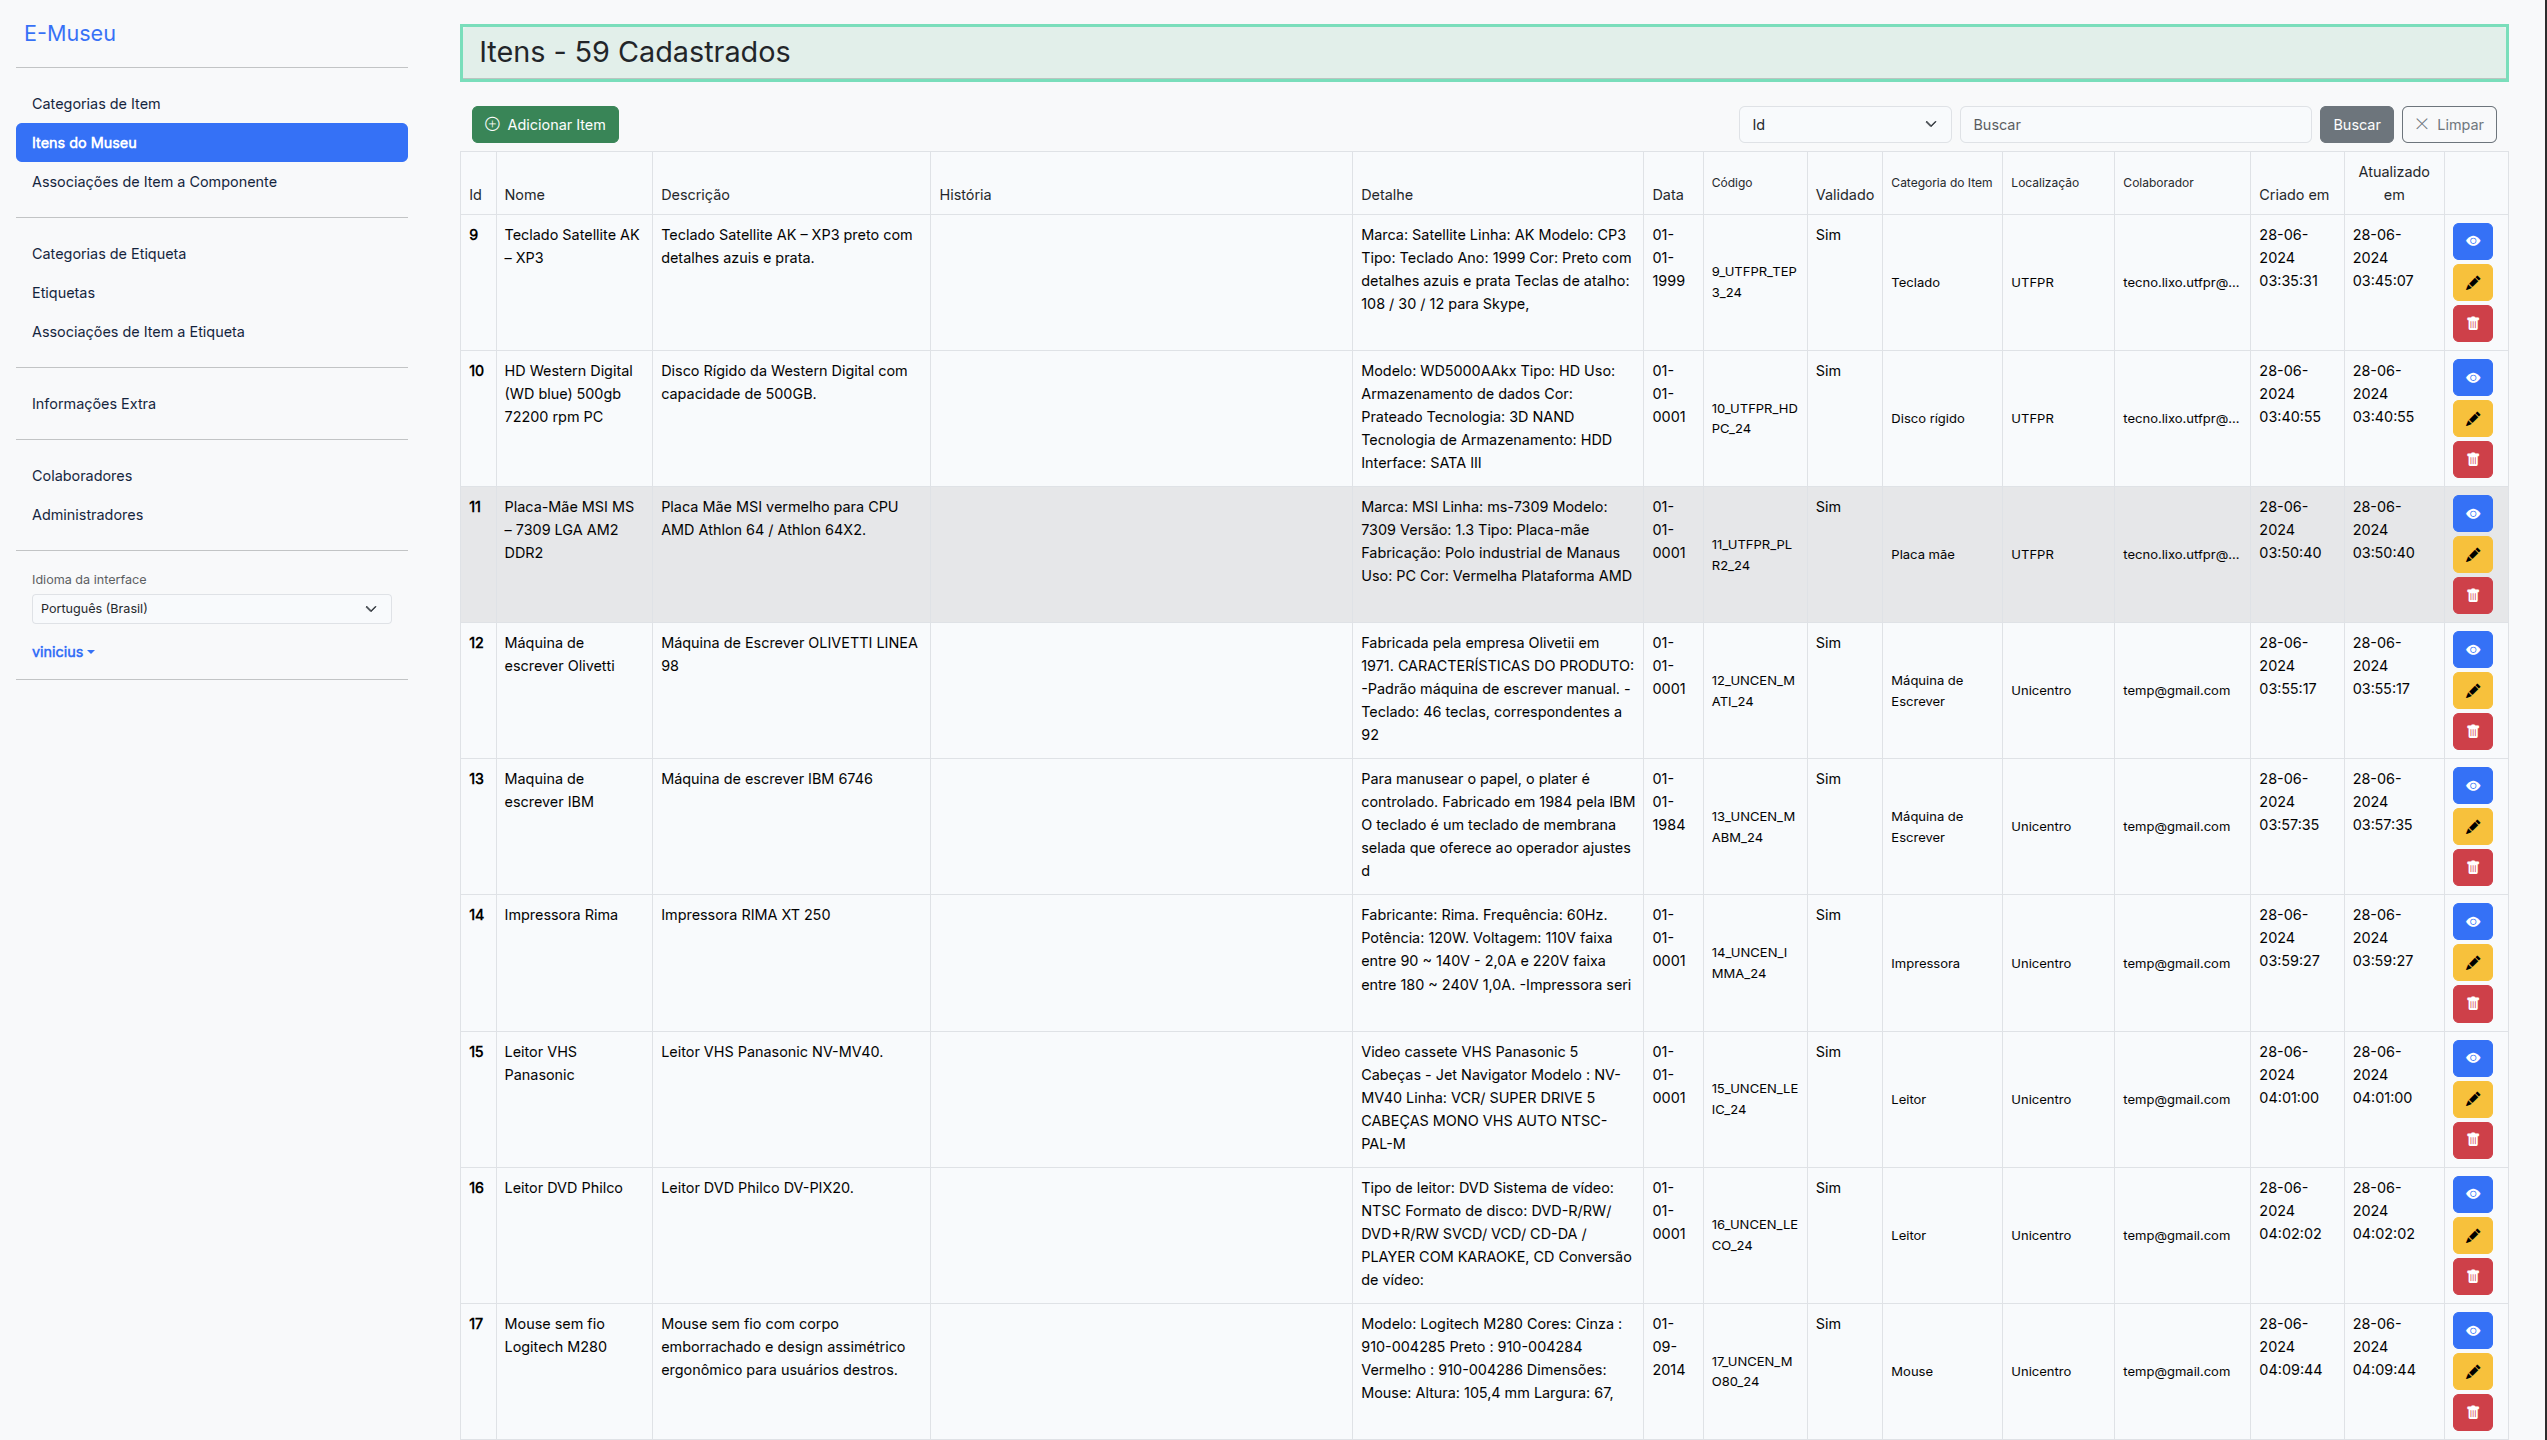
\includegraphics[width=\textwidth]{figuras/emuseu-admin.png}
    \caption{Painel administrativo: listagem de itens do acervo (\url{https://e-museu.gp.utfpr.edu.br/admin/catalog/items}).}
    \label{fig:emuseu-admin}
    \caption*{\textbf{Fonte:} Autoria própria (produção, maio/2026).}
\end{figure}


\section{Indicadores quantitativos do repositório}\label{sec:resultados-indicadores}

Os indicadores abaixo foram obtidos em maio de 2026 a partir do repositório institucional \texttt{e-museu-utfpr-gp/e-museu} e da linha legada usada para comparação (Tankensho), sem incluir dependências de terceiros (\texttt{vendor/}, \texttt{node\_modules/}). Servem como ordem de grandeza da ampliação do esforço de engenharia; contagens locais (arquivos em \texttt{tests/} ou linhas em \texttt{app/}) podem ser recalculadas com \texttt{cloc} ou \texttt{git diff --stat} entre \textit{tags}.

A Figura~\ref{fig:github-contribuicoes} reproduz a visão \textit{Contributors} do \textit{GitHub} para o ramo \texttt{main} (commits por semana, excluindo commits de \textit{merge}), disponível em \url{https://github.com/e-museu-utfpr-gp/e-museu/graphs/contributors?all=1}. O gráfico superior mostra dois momentos distintos: um pico em meados de 2024, quando o usuário \texttt{tankesho} concentrou a implementação inicial herdada do trabalho de \citeonline{gonzaga2024}; um intervalo com pouca atividade; e, a partir de janeiro de 2026, commits semanais contínuos até maio de 2026, período em que o autor desta monografia (\texttt{vinifen}) conduziu a refatoração, a infraestrutura e as funcionalidades documentadas no Capítulo~\ref{cap:desenvolvimento}. Nos cartões individuais, \texttt{vinifen} aparece com 116 commits e cerca de 86,9 mil linhas adicionadas e 47,5 mil removidas; \texttt{tankesho}, com 66 commits e cerca de 29,3 mil adições e 4,9 mil remoções. Esses totais incluem todo o histórico visível no repositório da organização (incluindo o período anterior ao \textit{fork} institucional em fevereiro de 2026) e não se limitam ao ciclo do TCC~2, mas ajudam a situar a magnitude do código sob \texttt{main} frente ao legado.

\begin{figure}[H]
    \centering
    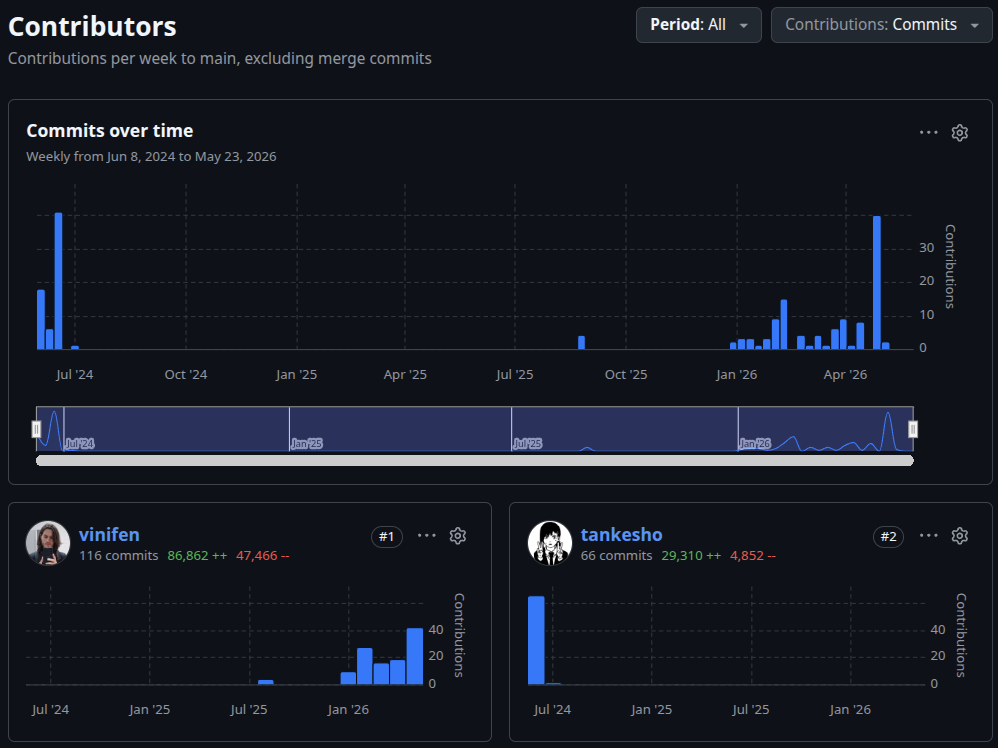
\includegraphics[width=\textwidth]{figuras/github-contribuições.png}
    \caption{Contribuições por commit no repositório \texttt{e-museu-utfpr-gp/e-museu} (ramo \texttt{main}).}
    \label{fig:github-contribuicoes}
    \caption*{\textbf{Fonte:} \textit{GitHub Insights -- Contributors} (\url{https://github.com/e-museu-utfpr-gp/e-museu/graphs/contributors?all=1}), captura de maio/2026.}
\end{figure}

\begin{itemize}
    \item \textit{Pull requests} documentados no histórico do TCC~2: 56 entregas exportadas do \textit{GitHub} da organização \texttt{e-museu-utfpr-gp} (arquivo de apoio do autor, maio/2026).
    \item Arquivos de teste PHP em \texttt{tests/}: 2 no legado; 92 na versão refatorada (inclui testes de fluxo, integração e unidade adicionados entre março e abril de 2026).
    \item Linhas em arquivos \texttt{.php} sob \texttt{app/}: aproximadamente 3,3 mil no legado; aproximadamente 13,8 mil na versão refatorada. O aumento reflete novos domínios, serviços e políticas de validação, não apenas cópia do código antigo.
    \item \textit{Releases} SemVer em \texttt{main}: \texttt{2.0.0-beta} e \texttt{2.1.0-beta} (infraestrutura e qualidade); \texttt{3.0.0-beta} (domínios, MinIO e base Laravel~12); \texttt{4.0.0-beta} (vocabulário do banco, \texttt{item\_images} e camada de serviços); \texttt{5.0.0-beta} (7 de abril de 2026) e \texttt{1.0.0} (25 de abril de 2026), com internacionalização, \texttt{Location}, Turnstile, tradução assistida e Laravel~13 (Capítulo~\ref{cap:desenvolvimento}).
    \item Atividade em \texttt{main} no \textit{GitHub} (Figura~\ref{fig:github-contribuicoes}): pico de commits em maio de 2026, alinhado ao encerramento da implantação institucional (Seção~\ref{sec:dev-deploy}).
\end{itemize}


\section{Entrega operacional}\label{sec:resultados-operacional}

O sistema encontra-se publicado em \url{https://e-museu.gp.utfpr.edu.br}, com validação prévia em \url{https://staging.e-museu.gp.utfpr.edu.br}. O ciclo de promoção (\textit{staging} antes de \texttt{main}), a infraestrutura Docker/Coolify e os artefatos de continuidade (sem exposição de credenciais neste documento) estão descritos nas Seções~\ref{sec:dev-deploy} e~\ref{sec:dev-infra}. Em síntese, a entrega reúne as condições para manutenção e evolução por quem assumir o projeto na instituição, sem depender da estrutura monolítica e pouco testada da implementação anterior.
